\documentclass[12pt]{article}

\usepackage{amsmath}
\usepackage{amssymb}
\usepackage{graphicx}
\usepackage{algorithm}% http://ctan.org/pkg/algorithms
\usepackage{algpseudocode}% http://ctan.org/pkg/algorithmicx
\usepackage{framed} % or, "mdframed"
\usepackage[framed]{ntheorem}
\usepackage{listings}
\newframedtheorem{frm-thm}{Lemma}

\usepackage[scale=1.0, left=1.0cm, right=1.0cm, top=1.865cm, bottom=0.865cm]{geometry}
\DeclareMathOperator*{\argmin}{arg\,min}

\pagestyle{myheadings}
\markright{CSE 260, Assignment 1 \hfill Andrew Conegliano, Matthias Springer\hfill}

\begin{document}

\title{Double-precision General Matrix Multiply (DGEMM)  \\ \vspace{2 mm} {\large Parallel Computation (CSE 260), Assignment 1}}
%\subtitle{Parallel Computation (CSE 260), Assignment 1}
\date{\today}
\author{Andrew Conegliano \and Matthias Springer}
\maketitle

\section{Introduction}

\subsection{Assumptions}
\begin{itemize}
	\item All matrices are square matrices.
	\item All matrices consist of double-precision floating point values (64-bit doubles).
\end{itemize}

\subsection{Notation}
In this work, we use the following notation and variable names.
\begin{itemize}
	\item $n$ is the size of one dimension of the matrices involved. I.e., every matrix has $n^2$ values.
	\item When referring to matrices, $A$ and $B$ denote the source matrices and $C$ denotes the target matrix, i.e. $AB = C$.
	\item $b_i$, $b_j$ and $b_k$ denote the block size for each \emph{dimension} $i$, $j$, and $k$, respectively\footnote{We tried multiple levels of blocking and it is evident from the context which level of blocking we are refering to.}.
\end{itemize}

\section{Hardware}

\section{Basic Algorithm}
The naive implementation of the matrix multiplication algorithm consists of three nested \lstinline{for} loops, where every loop runs from $1$ to $n$. In the innermost loop, a single addition and multiplication is done. Therefore, the runtime complexity of this algorithm is $\mathcal{O}(n^3)$ floating-point operations. We did not use an algorithm with a lower runtime complexity\footnote{Strassen's algorithm has a runtime complexity of $\mathcal{O}(n^{2.8})$.} because the idea of this assignment is to get familiar with memory access and caching. 

\section{Optimizations}

\subsection{Blocking for L1 Cache}

\subsection{Blocking for L2 Cache}
% theoretical explanation why it does not work

\subsection{Matrix Transposition}

\subsection{Register Blocking and Loop Unrolling}

\subsection{Matrix Buffering}

\subsection{Streaming SIMD Extensions (SSE)}
% + fused add multiply

\subsection{Parameter Tuning}
\subsubsection{Motivation}
As shown before, for certain matrix sizes $n$, the blocked algorithm performes better with certain block sizes. One obvious reason is that for a fixed matrix size $n$, the block size determines the size of the fringe cases. The code for fringe cases is less optimized than the code for regular cases and fringe cases might take less advantage of the cache. Also remember, that a cache line is $64$ bytes long and the size of a fringe case might not be divisible by the cache line size, i.e. a cache line is eventually not filled entirely with data from the fringe case. Therefore, we want to keep the fringe cases as small as possible. Let $f_i$ be the size of the fringe cases in dimension $i$\footnote{The same argument applies for the other dimensions.}. 

$$f_i = n \mod b_i$$

For example, for $n=372$, $b_i=16$ might be a better block size than $b_i=32$, because it results in fringe cases of size $4$ instead of $20$.

\subsubsection{Search Space}
We tried values for $b_i$, $b_j$ and $b_k$ for the L1 cache blocking. Due to certain implementation details, $b_i$ and $b_j$ must always be the same value. A cache line is $64$ bytes ($8$ doubles) long. Therefore, in order to reduce the search space, it makes sense to only take a look at multiples of $8$. We tried all possible combinations of $b_i=b_j, b_k \in \{8, 16, 24, 32, 40, 48, 56, 64\}$, resulting in $64$ parameter combinations. We ran the program for every matrix size from $n=10$ to $n=1200$. For every value of $n$, we then selected the parameters $b_i$ and $b_k$ with the highest performance. 

\subsubsection{Implementation}
We hard-coded the block size parameters for all matrix sizes from $n=10$ to $n=1200$. Based on the matrix size, a different version of the algorithm with the respective block size is run. For all other matrix sizes, we use $b_i=b_j=8$, $b_k=64$, because it performed good on average.

\subsubsection{Results and Evaluation}
\begin{figure}
	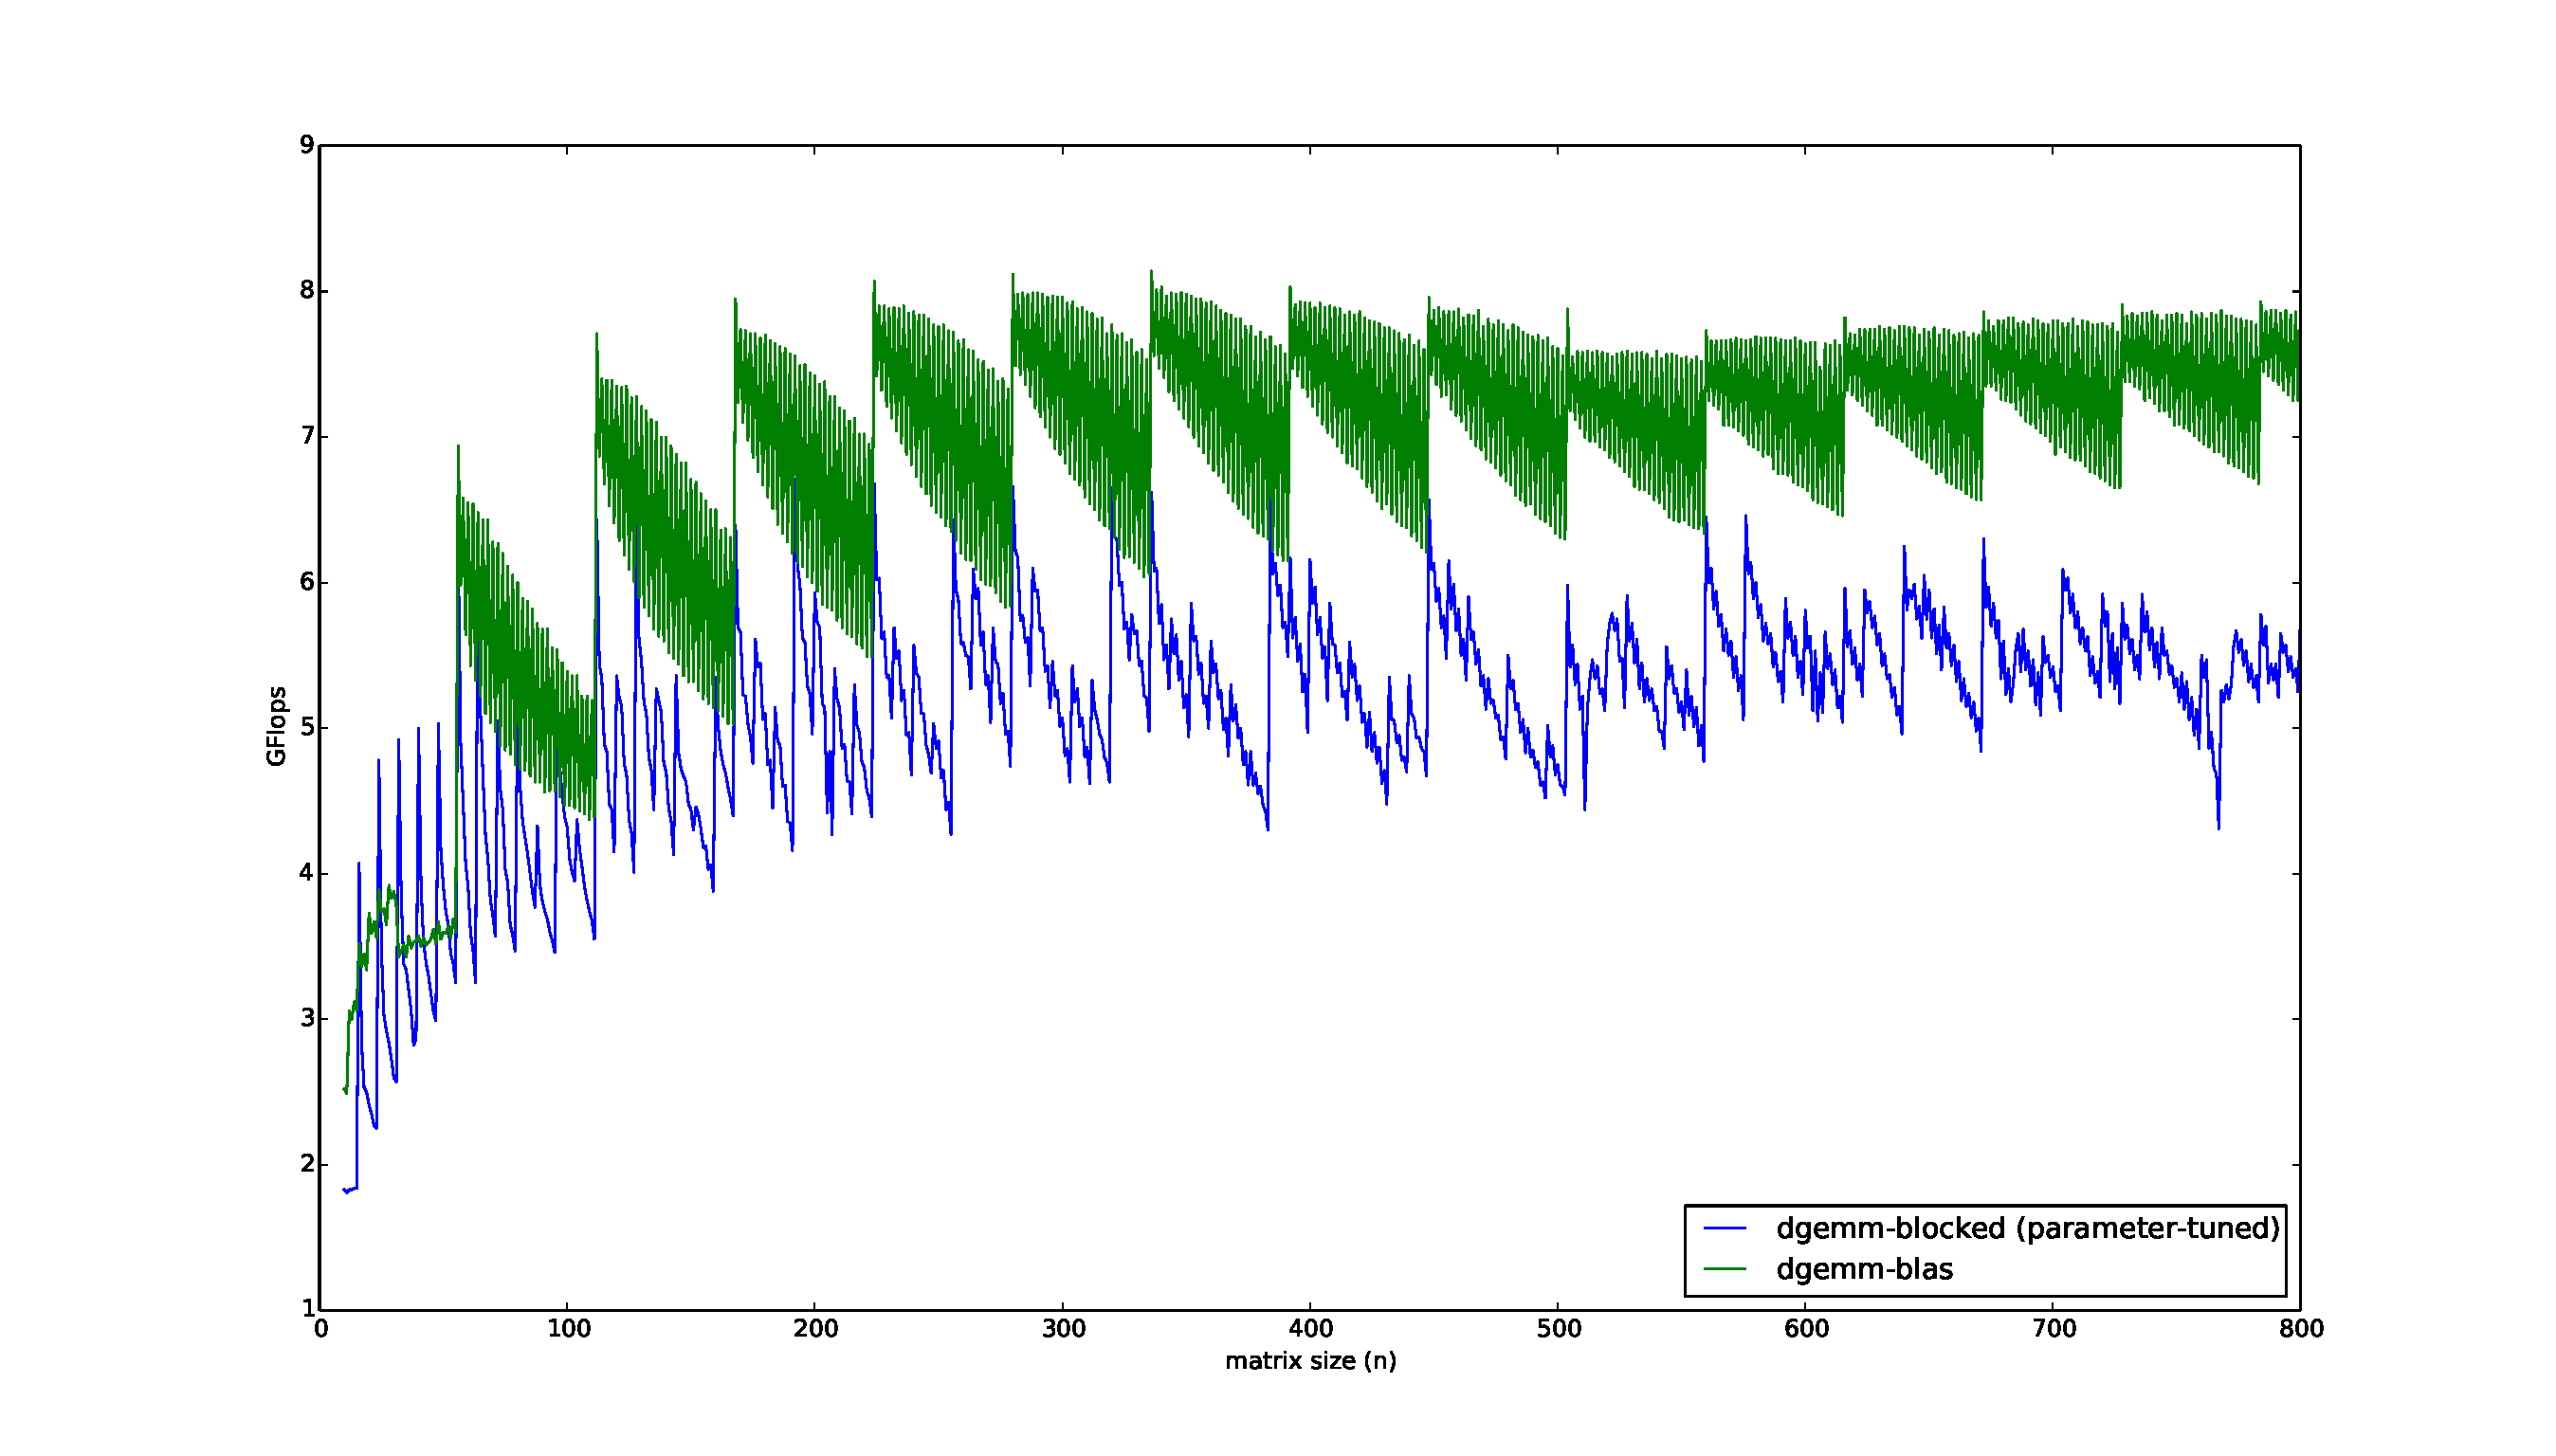
\includegraphics[width=\textwidth]{graphs/profiles/PROFILE_BLOCKED.pdf}
	\caption{Performance of our parameter-tuned blocking version, in comparison to ATLAS.}
\end{figure}

\section{Performance Evaluation}
\subsection{Parameter Tuning}

\newpage
\section*{Appendix}
\subsection*{Performance Tuning}
%\begin{tabular}{cccc}
	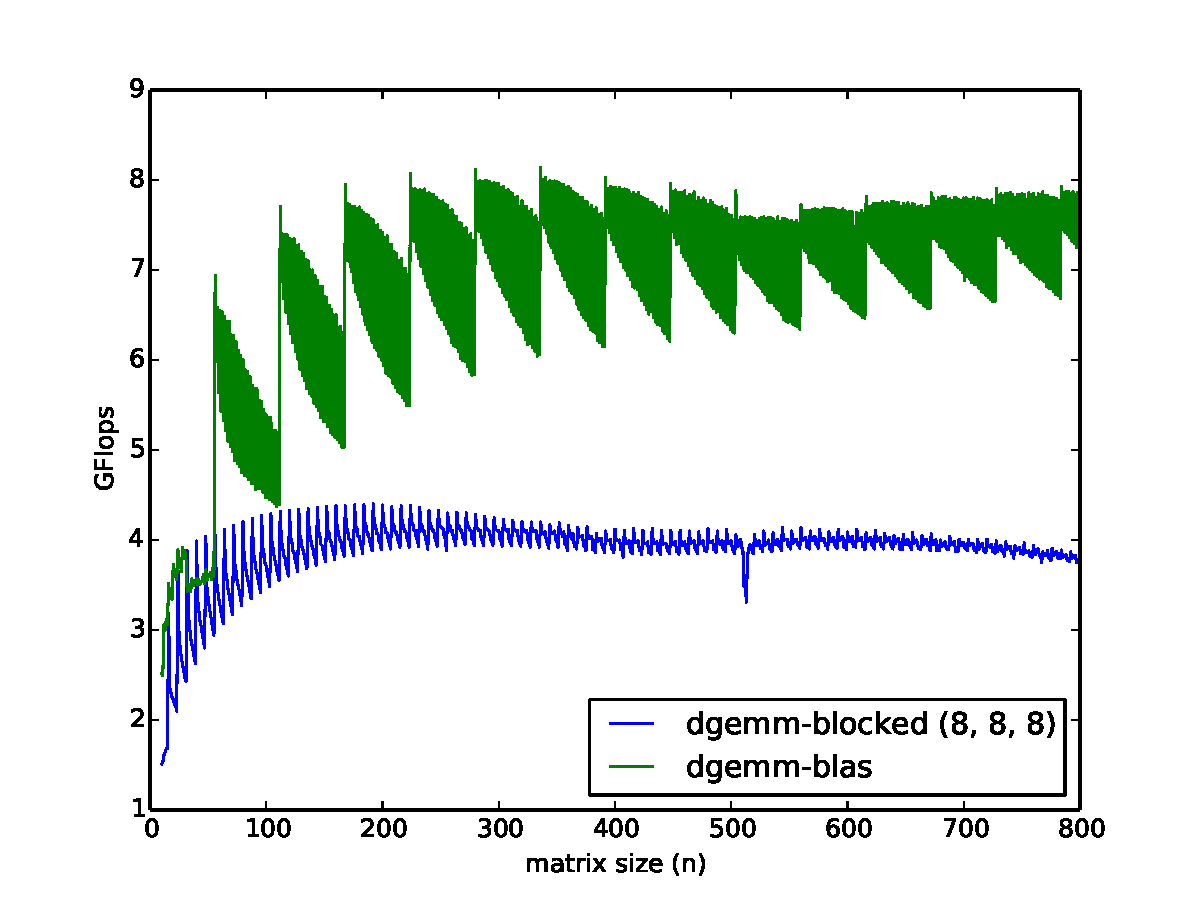
\includegraphics[width=0.25\textwidth]{graphs/profiles/PROFILE_OUTUT_8_8.pdf}  
	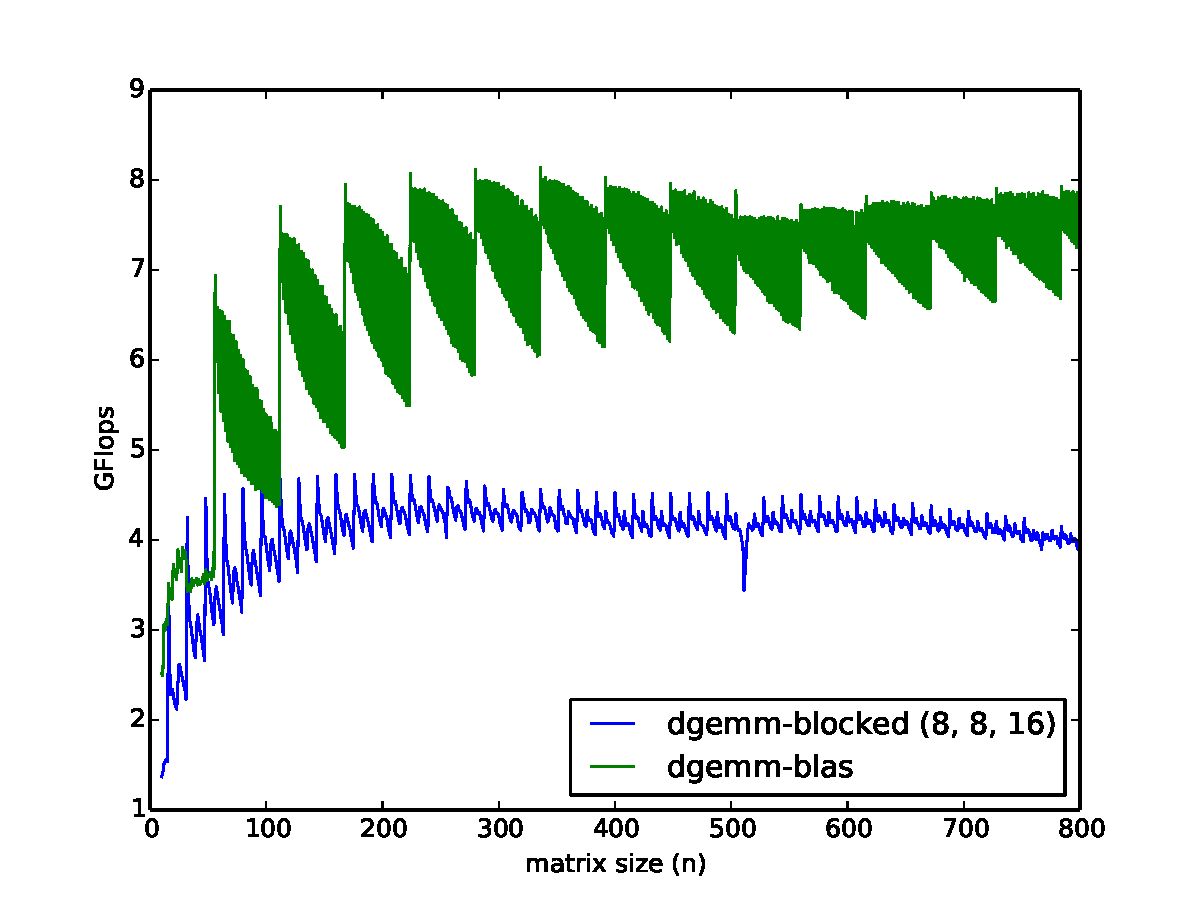
\includegraphics[width=0.25\textwidth]{graphs/profiles/PROFILE_OUTUT_8_16.pdf}  
	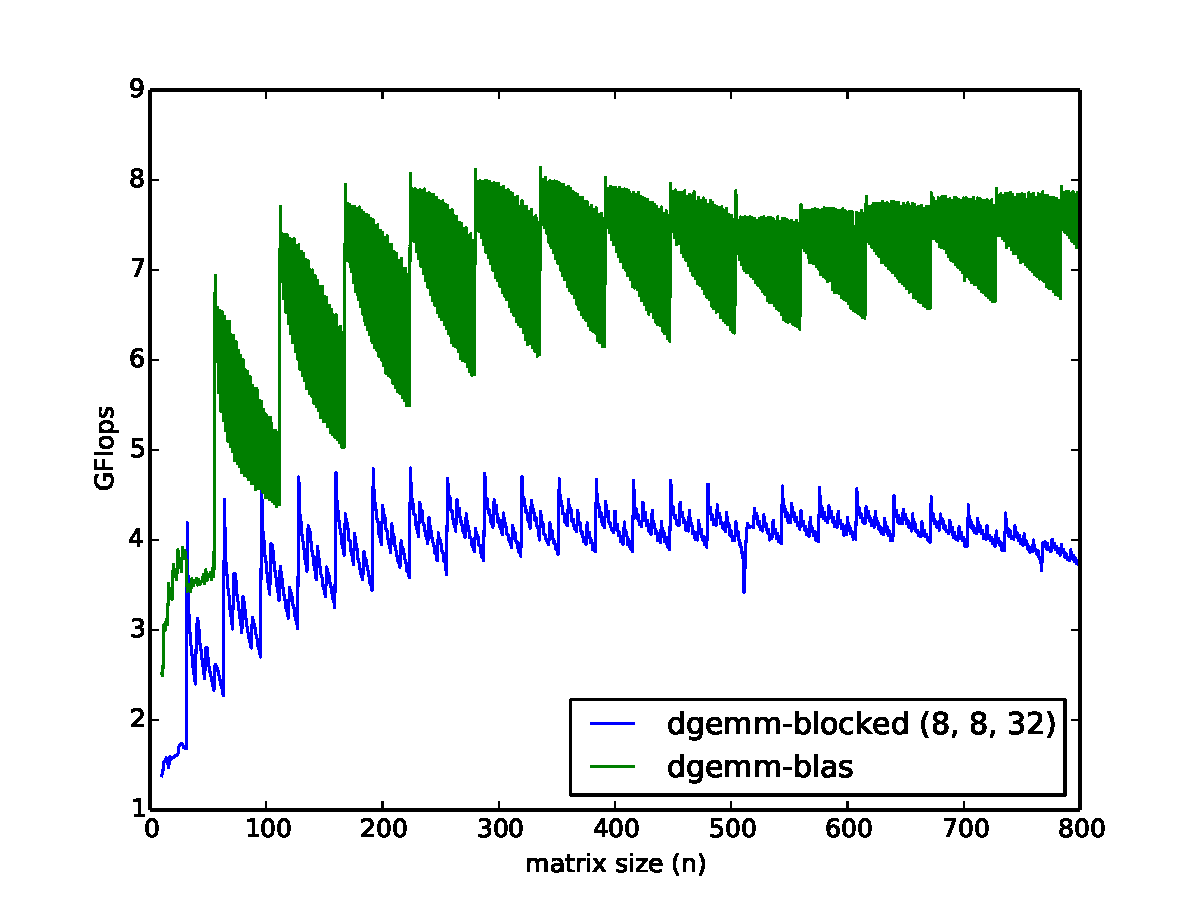
\includegraphics[width=0.25\textwidth]{graphs/profiles/PROFILE_OUTUT_8_32.pdf} 
	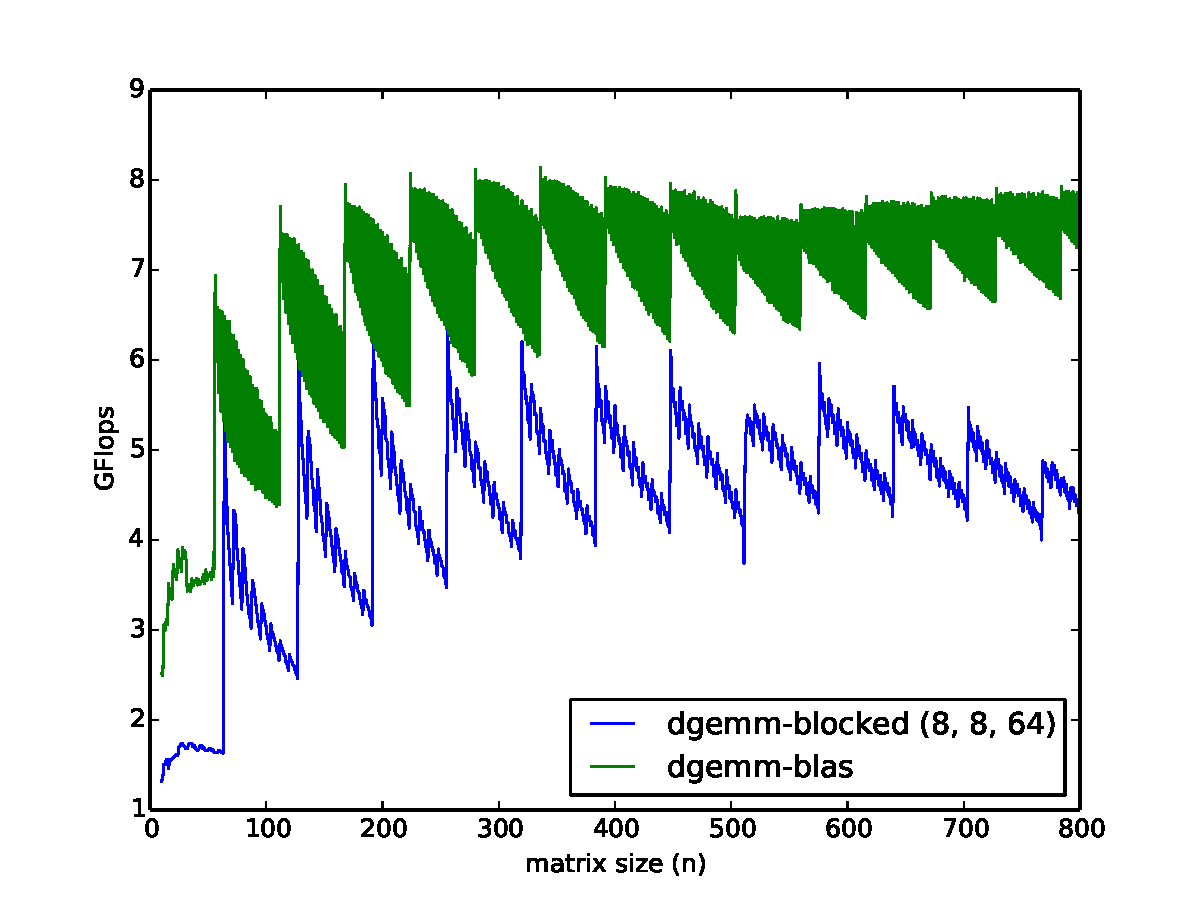
\includegraphics[width=0.25\textwidth]{graphs/profiles/PROFILE_OUTUT_8_64.pdf} 
	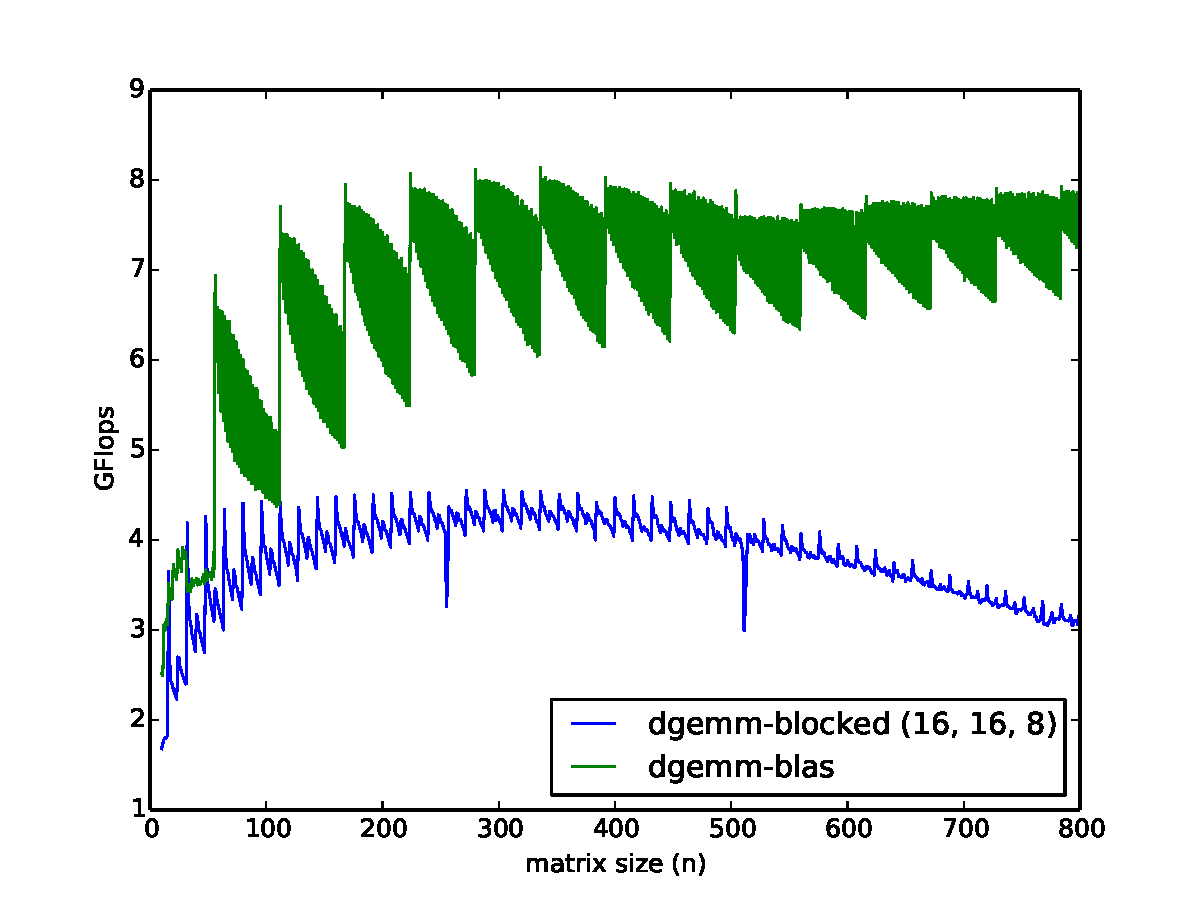
\includegraphics[width=0.25\textwidth]{graphs/profiles/PROFILE_OUTUT_16_8.pdf}  
	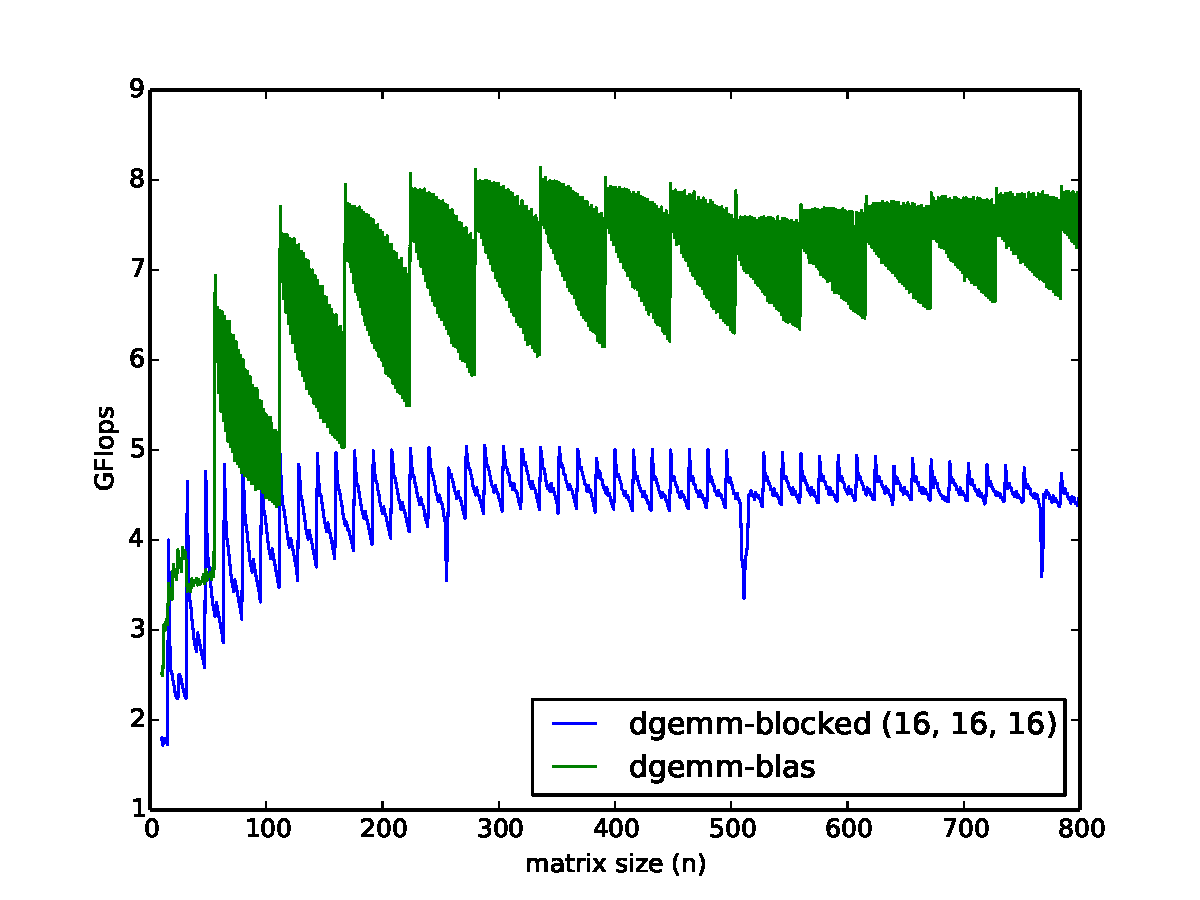
\includegraphics[width=0.25\textwidth]{graphs/profiles/PROFILE_OUTUT_16_16.pdf}  
	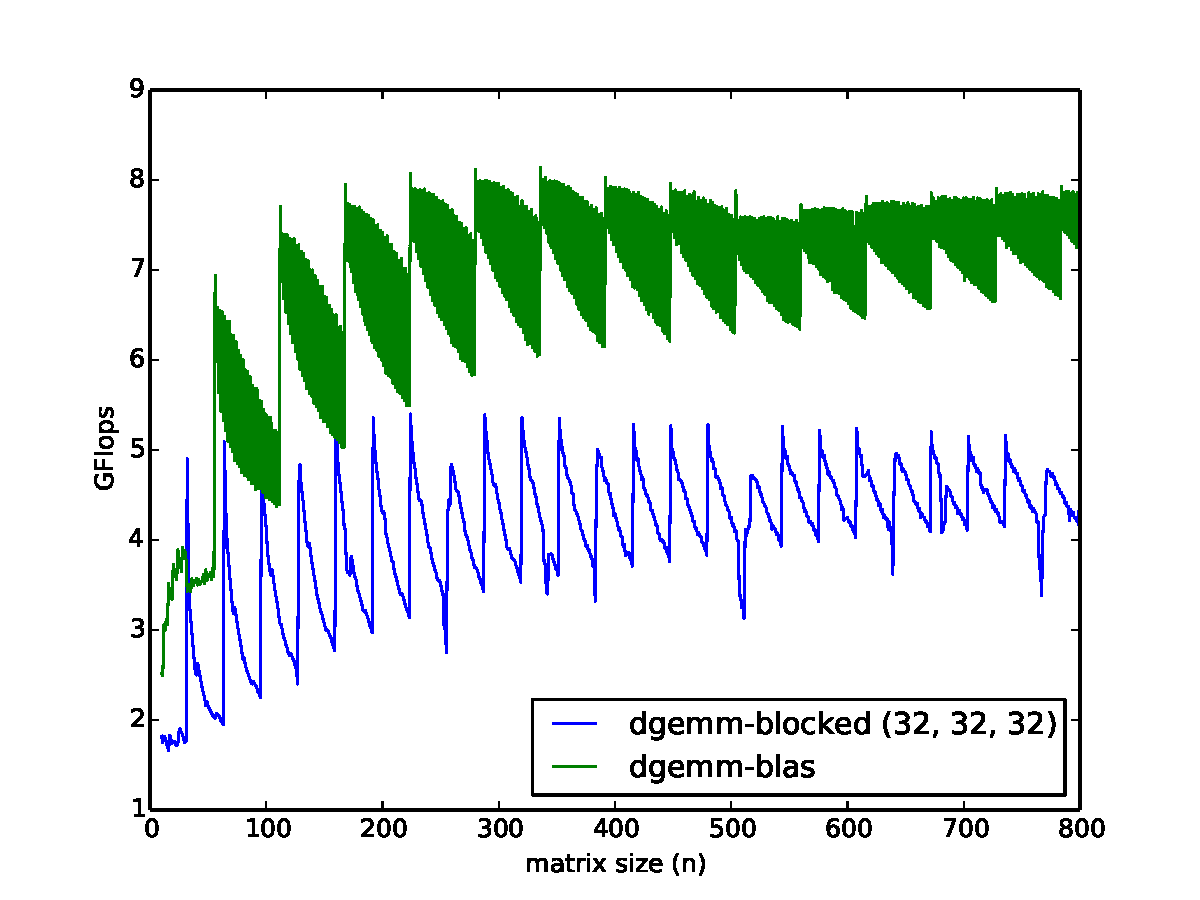
\includegraphics[width=0.25\textwidth]{graphs/profiles/PROFILE_OUTUT_32_32.pdf} 
	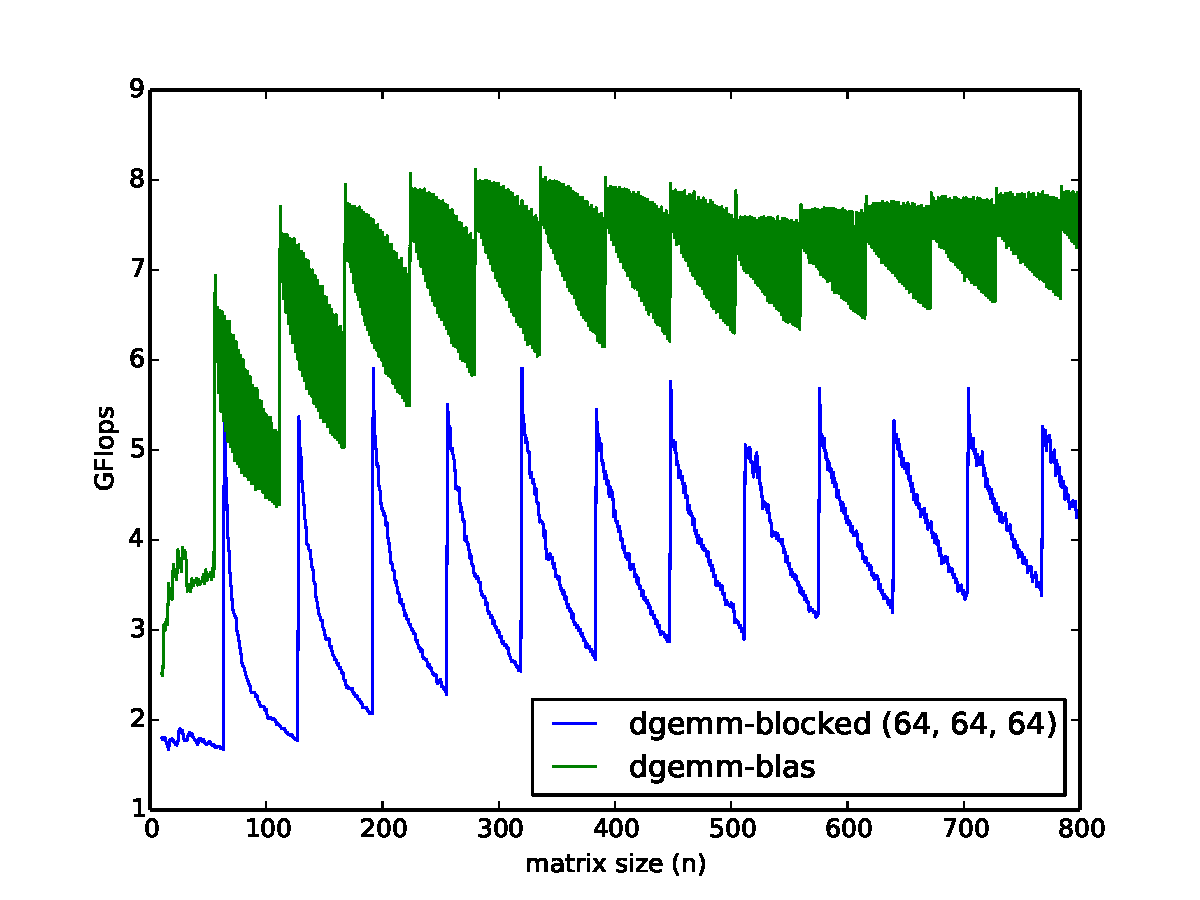
\includegraphics[width=0.25\textwidth]{graphs/profiles/PROFILE_OUTUT_64_64.pdf} 
	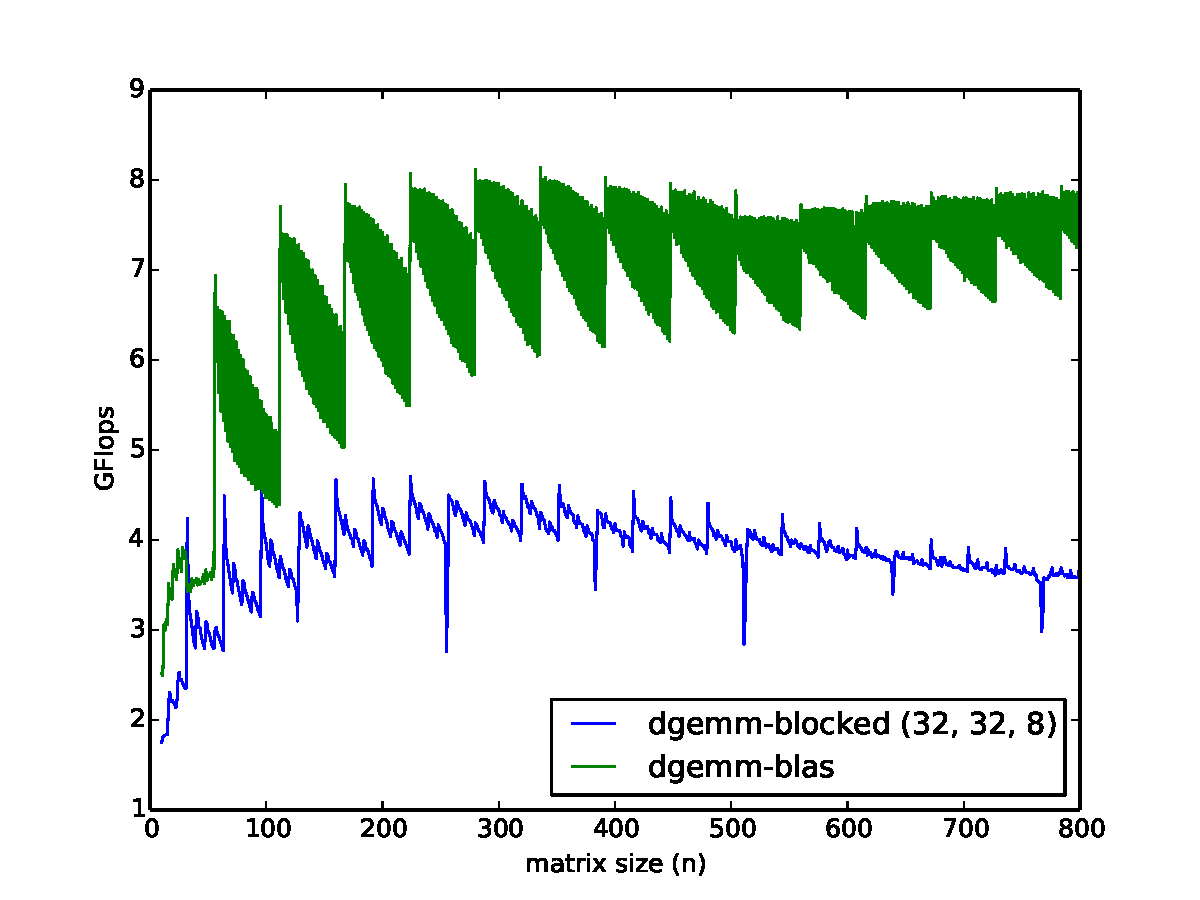
\includegraphics[width=0.25\textwidth]{graphs/profiles/PROFILE_OUTUT_32_8.pdf}  
	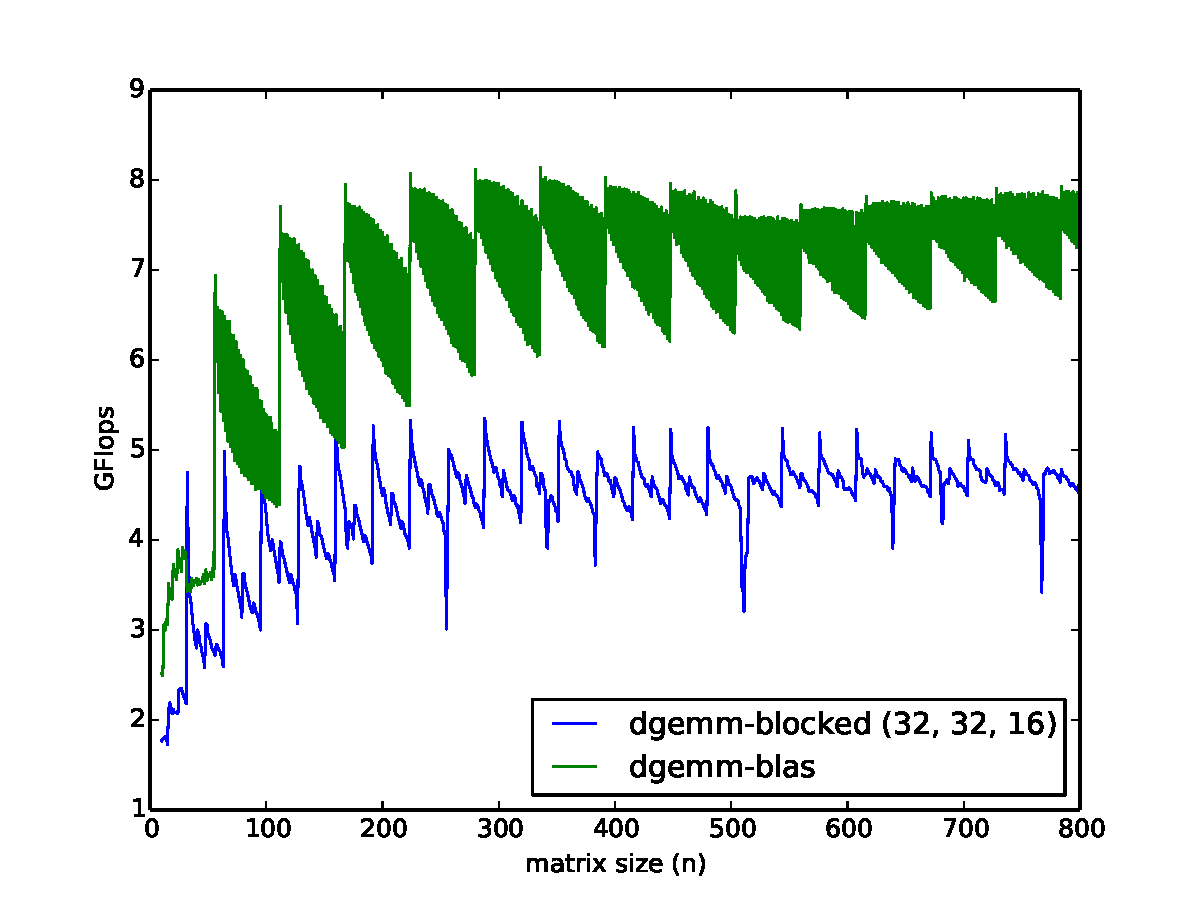
\includegraphics[width=0.25\textwidth]{graphs/profiles/PROFILE_OUTUT_32_16.pdf}  
	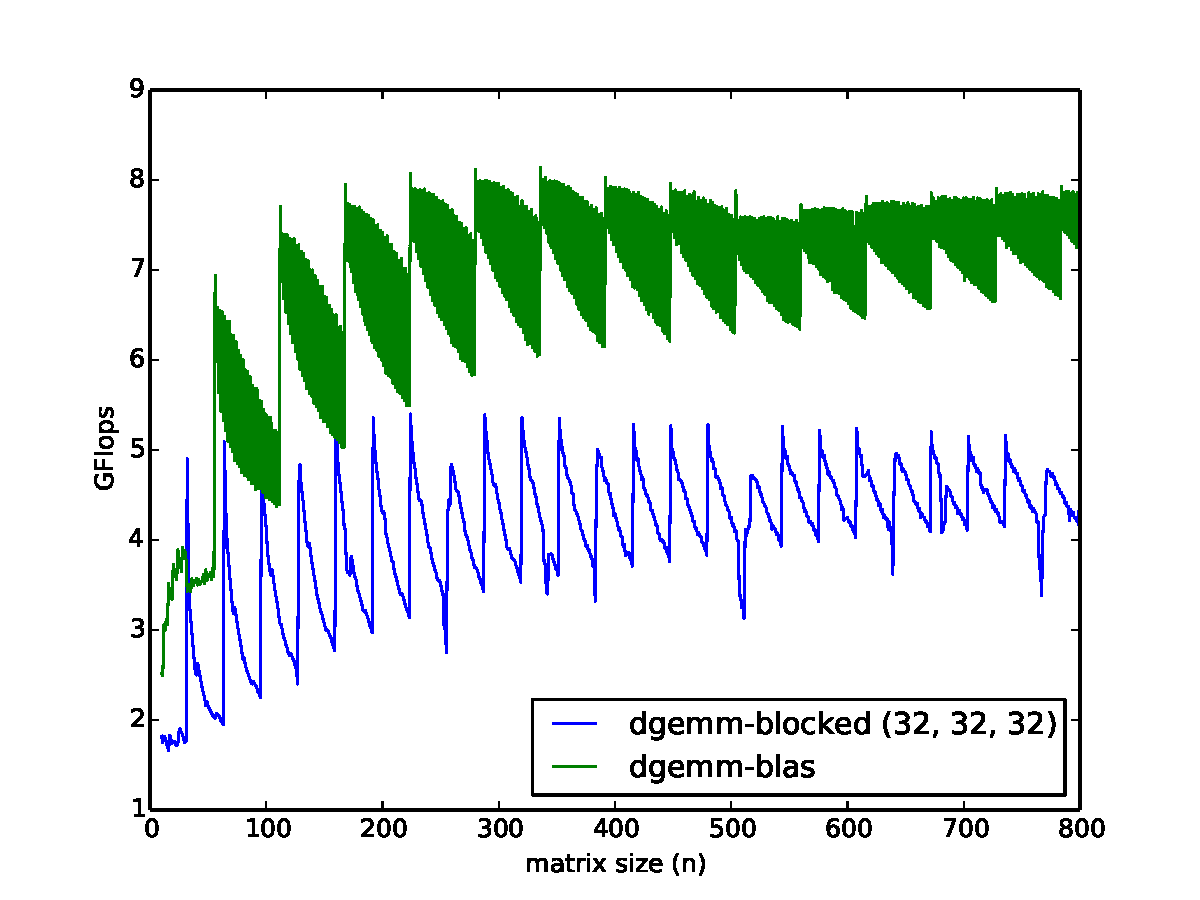
\includegraphics[width=0.25\textwidth]{graphs/profiles/PROFILE_OUTUT_32_32.pdf} 
	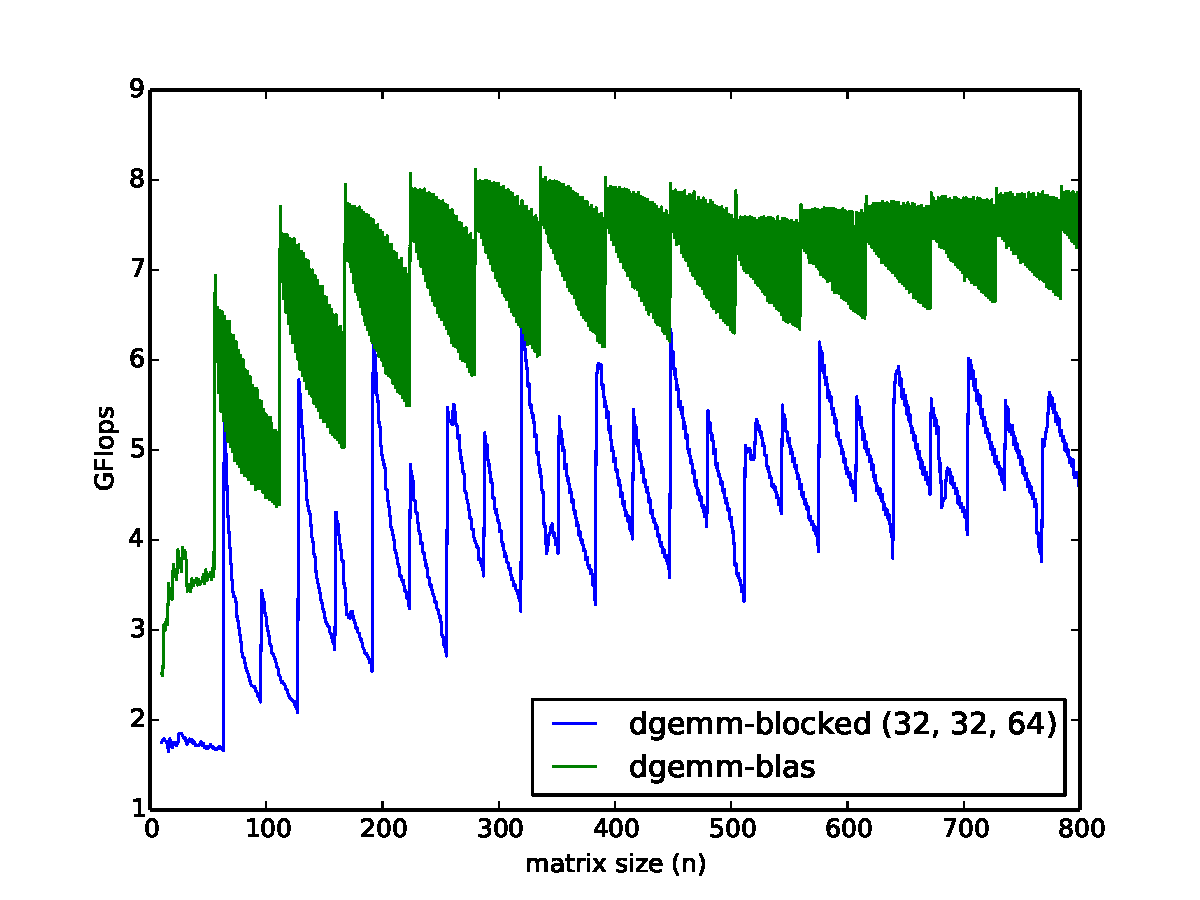
\includegraphics[width=0.25\textwidth]{graphs/profiles/PROFILE_OUTUT_32_64.pdf} 
	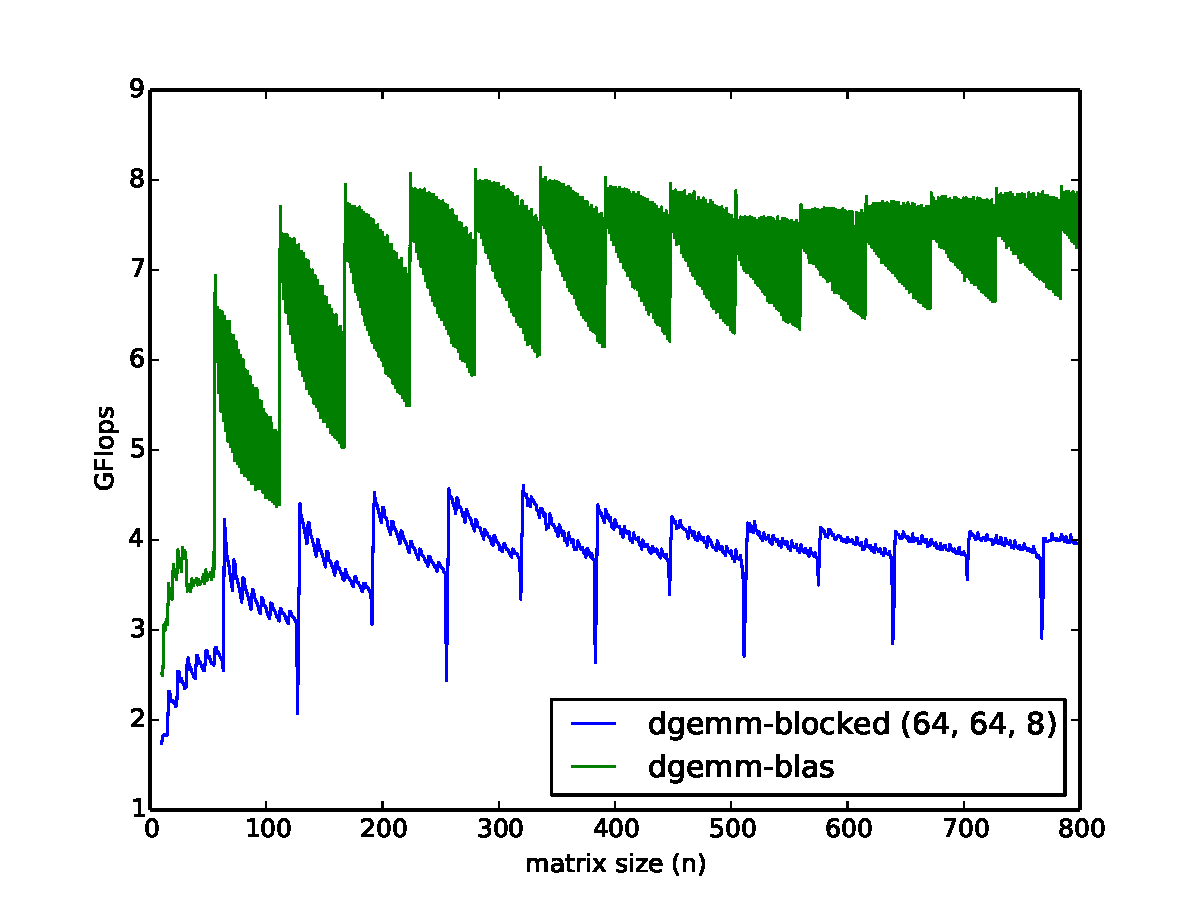
\includegraphics[width=0.25\textwidth]{graphs/profiles/PROFILE_OUTUT_64_8.pdf}  
	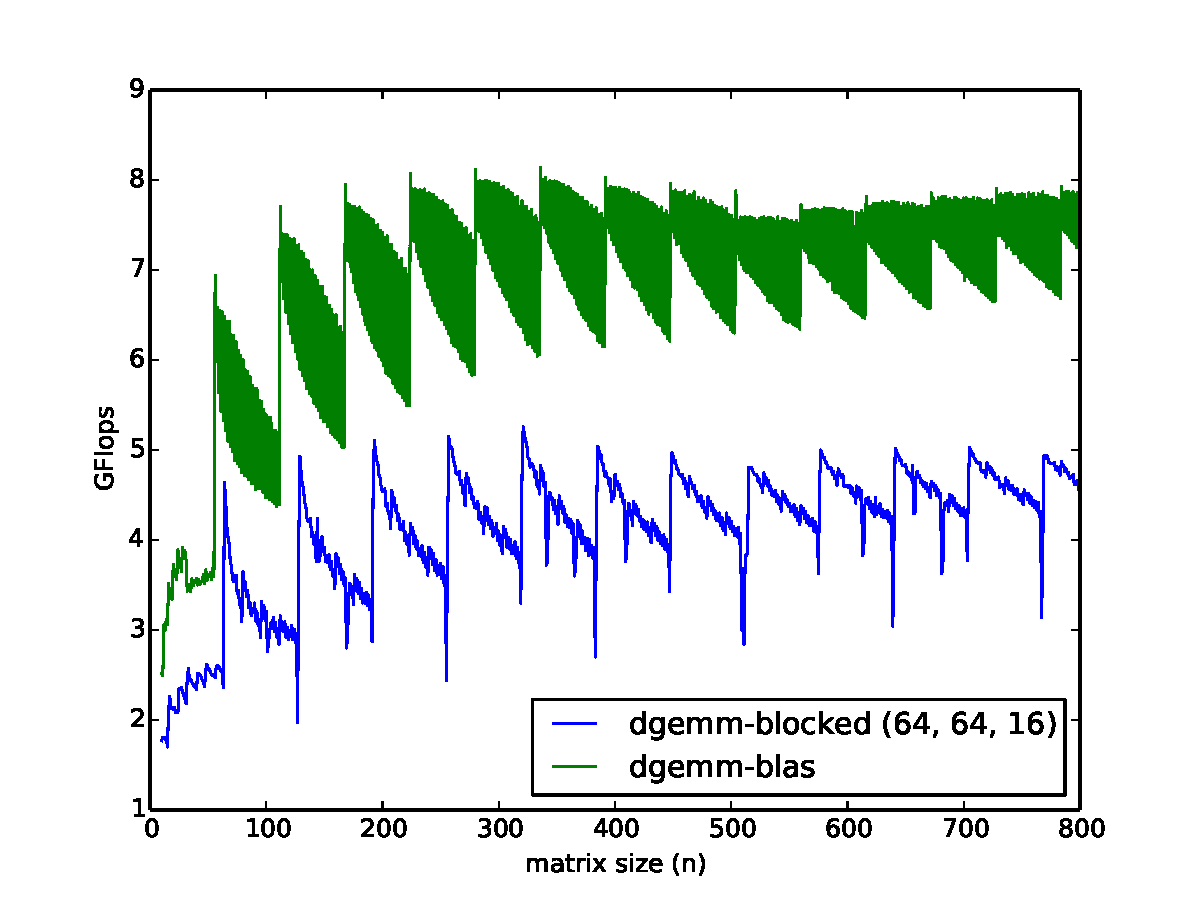
\includegraphics[width=0.25\textwidth]{graphs/profiles/PROFILE_OUTUT_64_16.pdf}  
	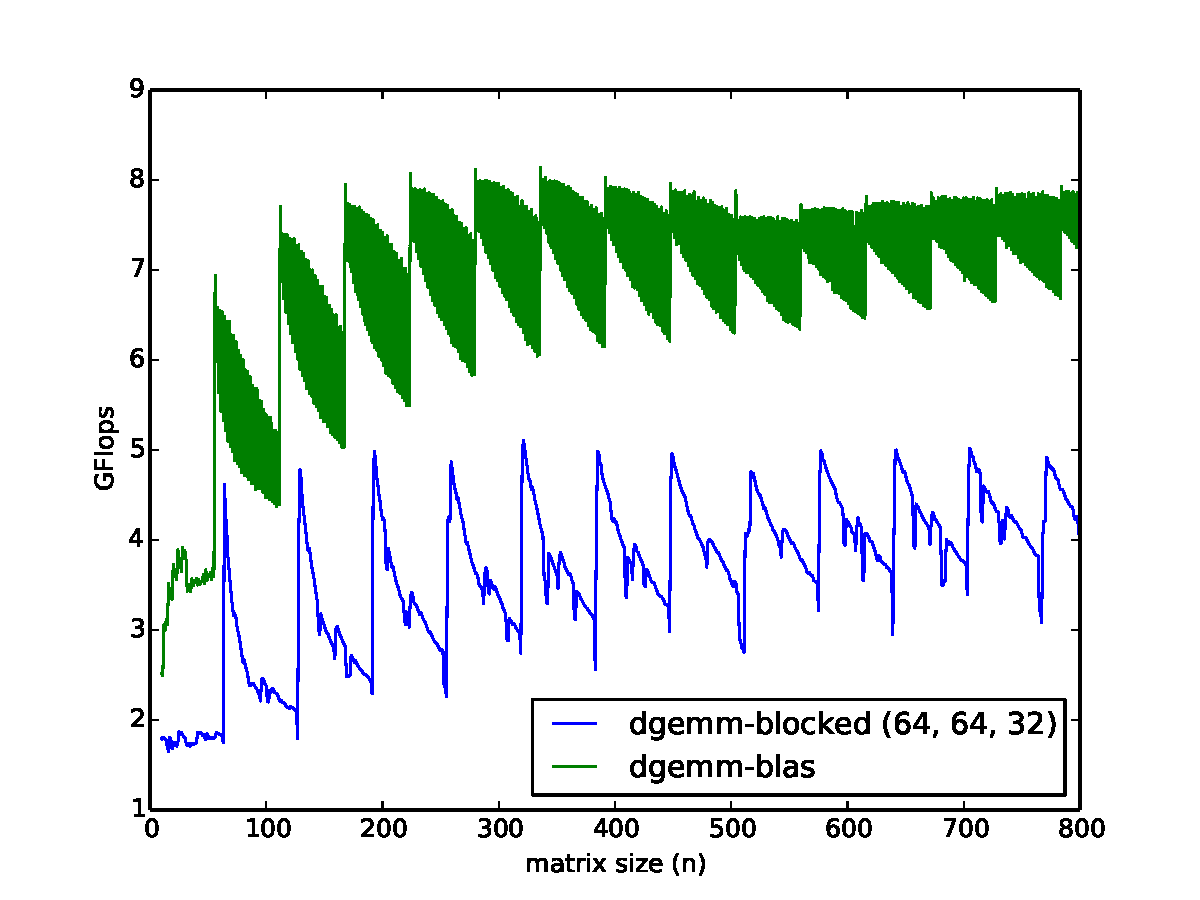
\includegraphics[width=0.25\textwidth]{graphs/profiles/PROFILE_OUTUT_64_32.pdf} 
	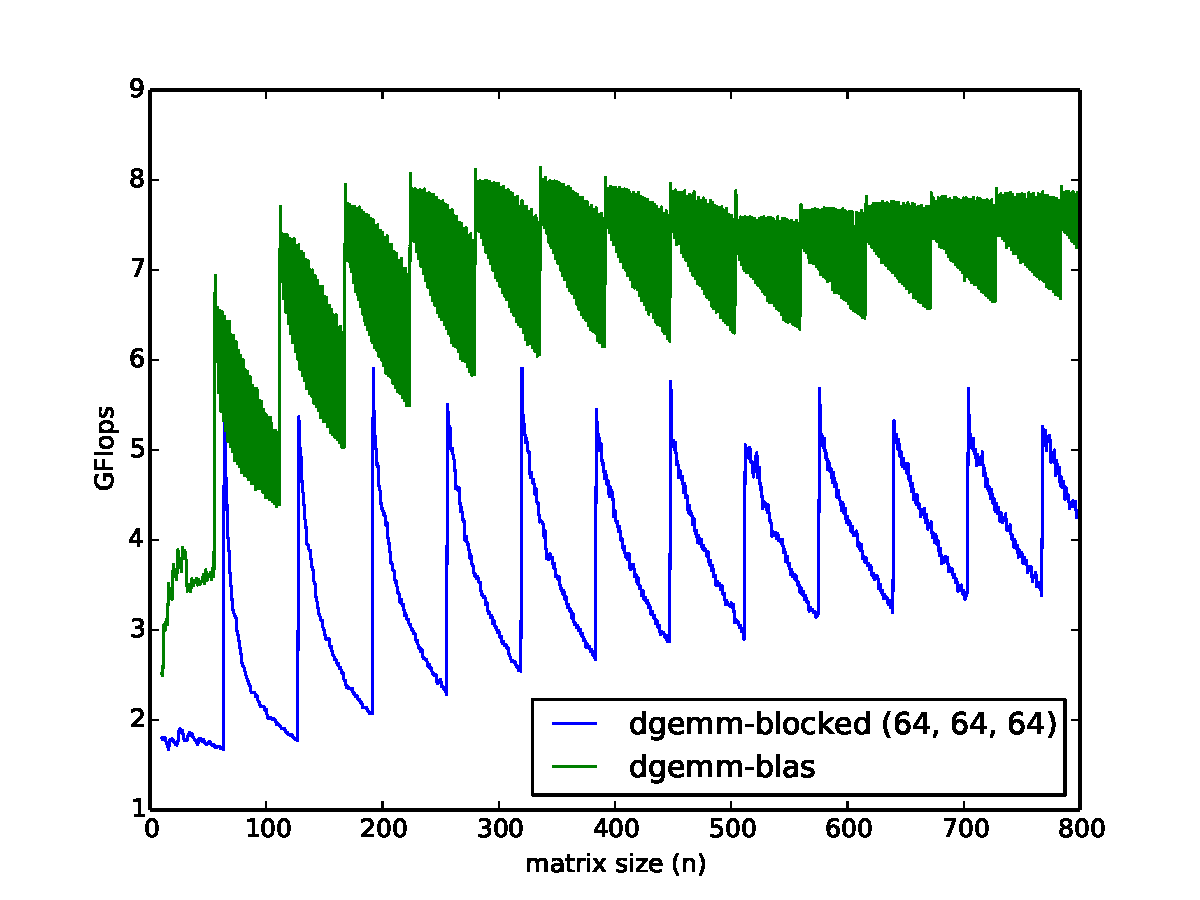
\includegraphics[width=0.25\textwidth]{graphs/profiles/PROFILE_OUTUT_64_64.pdf} 
	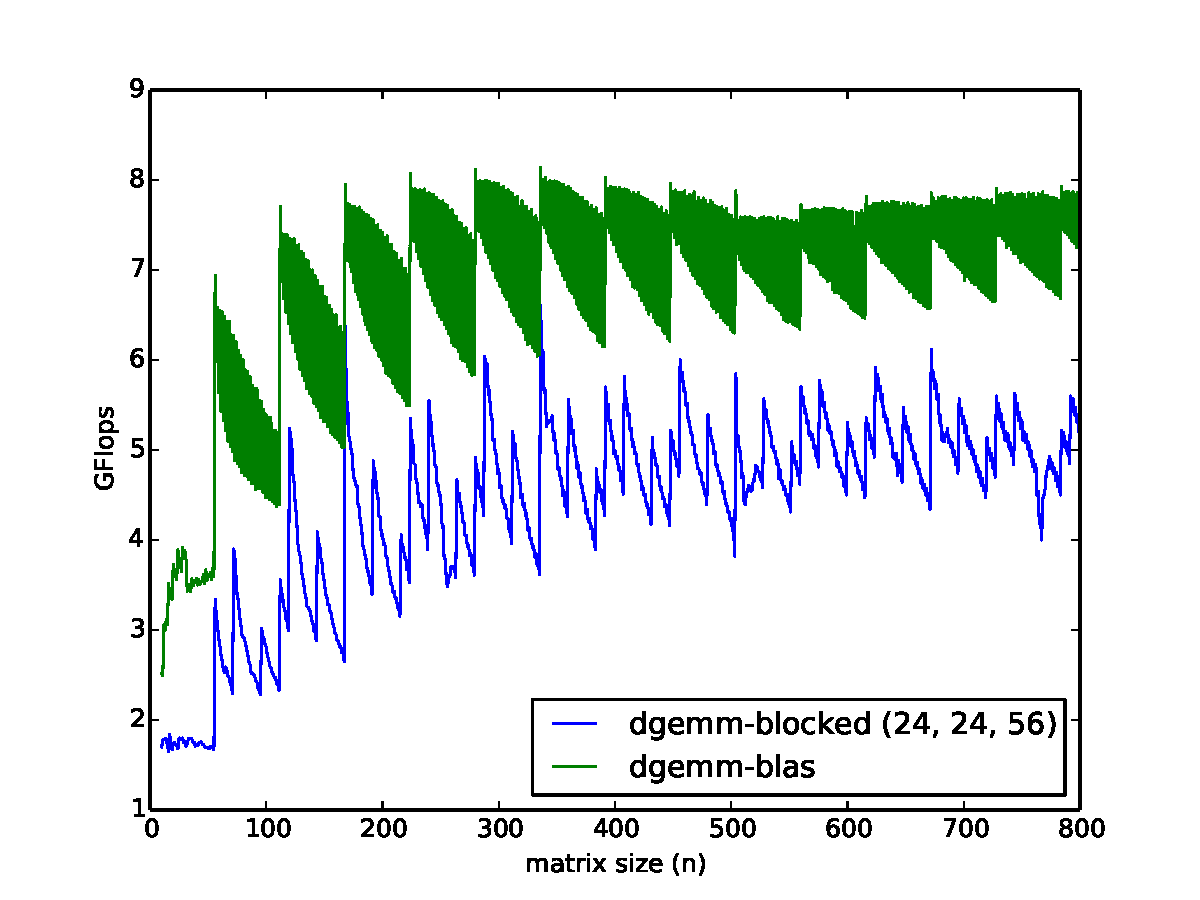
\includegraphics[width=0.25\textwidth]{graphs/profiles/PROFILE_OUTUT_24_56.pdf}  
	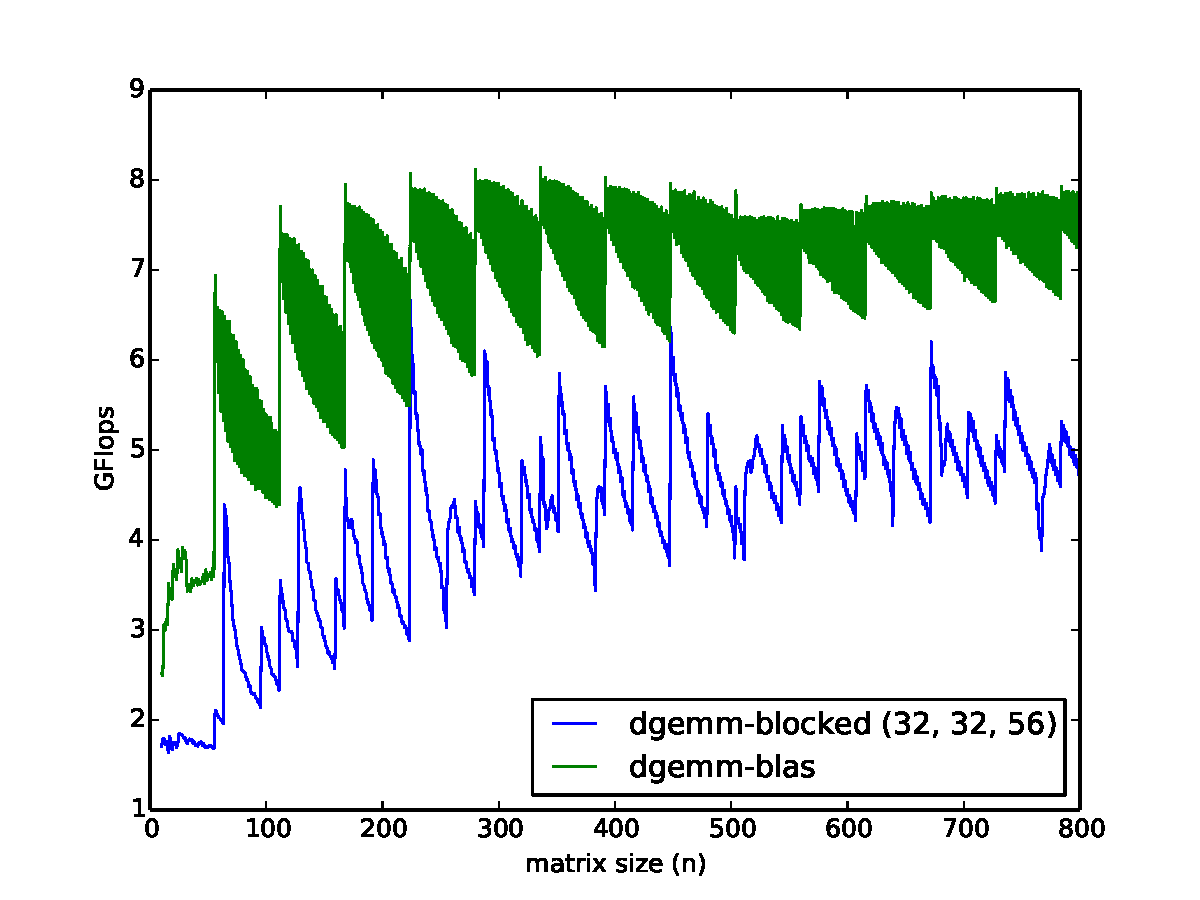
\includegraphics[width=0.25\textwidth]{graphs/profiles/PROFILE_OUTUT_32_56.pdf}  
	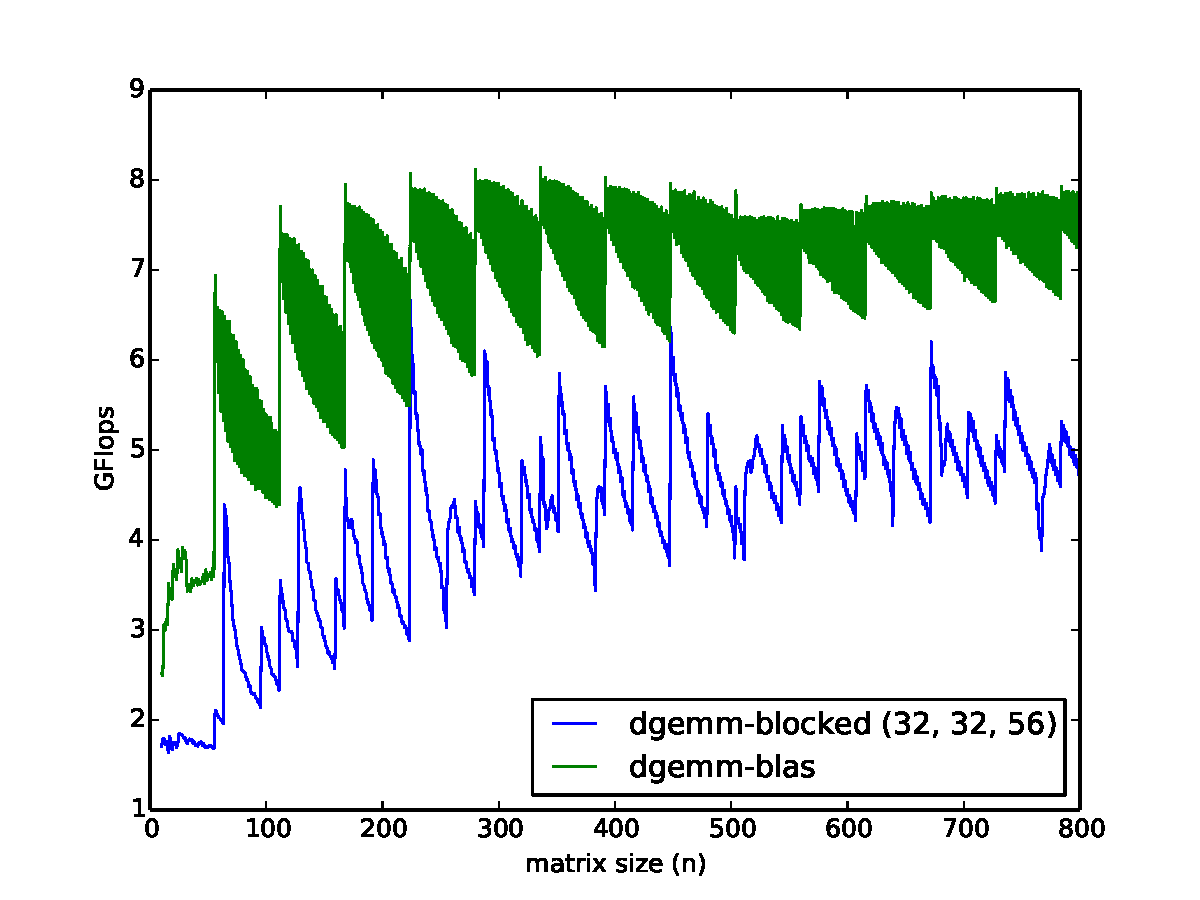
\includegraphics[width=0.25\textwidth]{graphs/profiles/PROFILE_OUTUT_32_56.pdf} 
	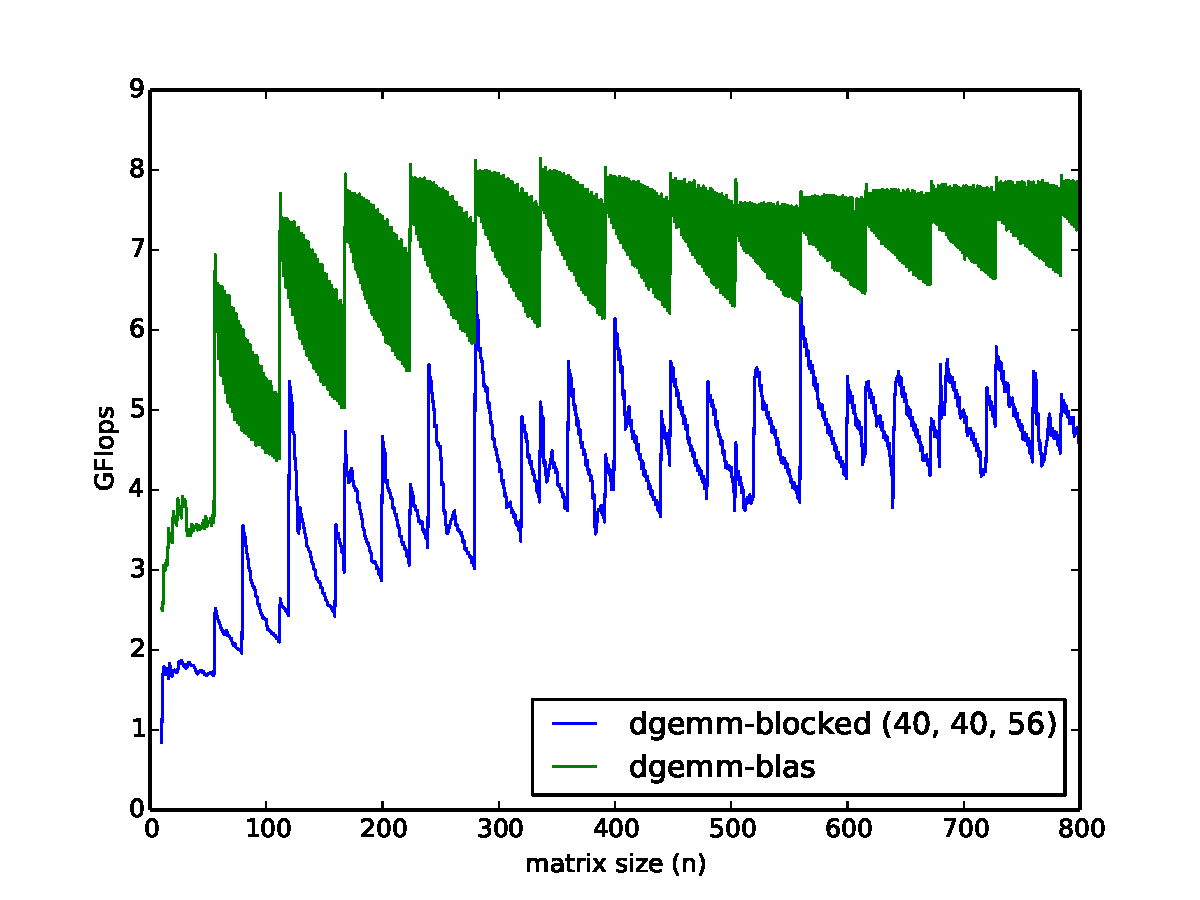
\includegraphics[width=0.25\textwidth]{graphs/profiles/PROFILE_OUTUT_40_56.pdf} 
%\end{tabular}
\end{document}

